\section{508 --- Most Frequent Subtree Sum}
Given the root of a tree, you are asked to find the most frequent subtree sum. The subtree sum of a node is defined as the sum of all the node values formed by the subtree rooted at that node (including the node itself). So what is the most frequent subtree sum value? If there is a tie, return all the values with the highest frequency in any order.

\paragraph{Examples 1}
\begin{flushleft}
\textbf{Input}:
\begin{figure}[H]
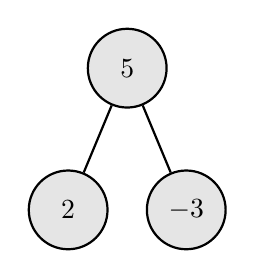
\begin{tikzpicture}
[every node/.style={draw, circle,
 minimum size=10mm, fill=gray!20!},
  level distance=18mm, 
 thick
]
\node{5}
	child{node{2}}
	child{node{$-3$}};
\end{tikzpicture}
\end{figure}
\textbf{Output}: $[2, -3, 4]$

\textbf{Explanation}:

Since all the values happen only once, return all of them in any order.
\end{flushleft}

\paragraph{Examples 2}
\begin{flushleft}
\textbf{Input}:
\begin{figure}[H]
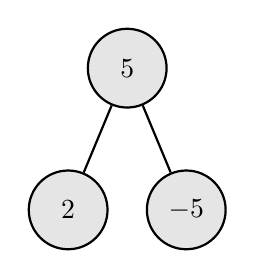
\begin{tikzpicture}
[every node/.style={draw, circle,minimum size=10mm, fill=gray!20!},level distance=18mm, thick
]
\node{5}
	child{node{2}}
	child{node{$-5$}};
\end{tikzpicture}
\end{figure}

\textbf{Output}: $[2]$

\textbf{Explanation}:

Since 2 happens twice, however $-5$ only occur once.
\end{flushleft}

\paragraph{Note:} 

\begin{itemize}
\item You may assume the sum of values in any subtree is in the range of 32-bit signed integer.
\end{itemize}

\subsection{Recursive}
\begin{itemize}
\item 对于每一个node,其total sum可分解为左右子树的sum加上其自身的value。
\item Maintain a hash map which maps the sum and the counts。
\item Maintain a variable, $x$, to track the maximum count of sums.
\end{itemize}

\setcounter{lstlisting}{0}
\begin{lstlisting}[style=customc, caption={Recursion}]
vector<int> findFrequentTreeSum( TreeNode* root )
{

    vector<int> ans;
    unordered_map<int, int> m;
    int max_count = 0;

    dfs( root, max_count, ans, m );

    return ans;
}
//recursion helper function
int dfs( TreeNode* node, int& max_count, vector<int>& ans, unordered_map<int, int>& m )
{
    if( !node )
    {
        return 0;
    }

    int sum = node->val;
    int left_sum = 0;


    //get left substree sum
    if( node->left )
    {
        left_sum = dfs( node->left, max_count, ans, m );
    }

    int right_sum = 0;

    //get right substree sum
    if( node->right )
    {
        right_sum = dfs( node->right, max_count, ans, m );
    }

    sum += left_sum;
    sum += right_sum;

    //track the maximum count of sums
    //and put (sum, count) into hash map
    int count = 1;
    auto it = m.find( sum );

    if( it != m.end() )
    {
        ++it->second;
        count = it->second;
    }
    else
    {
        m.emplace( sum, 1 );
    }

    if( count > max_count )
    {
        max_count = count;
        ans.clear();
        ans.push_back( sum );
    }
    else if( count == max_count )
    {
        ans.push_back( sum );
    }

    return sum;
}
\end{lstlisting}
